\chapter{HASIL DAN PEMBAHASAN}

\section{Hasil Perancangan Sistem Tertanam}
Hasil perancangan sistem tertanam berupa arsitektur kendali berbasis Raspberry Pi 5 yang menghubungkan kamera, \textit{pipeline} MediaPipe, modul pemilihan mode, dan dua robot manipulator. Sistem dibagi menjadi dua mode utama, yaitu mode pengenalan SIBI pada meArm dan mode teleoperasi pada Dobot Magician. Pembagian mode ini bertujuan agar satu perangkat komputasi dapat menjalankan dua fungsi interaksi manusia--robot yang berbeda.

Secara umum, alur sistem dimulai dari akuisisi citra tangan oleh kamera. Citra tersebut diproses oleh MediaPipe untuk menghasilkan \textit{landmark} tangan. \textit{Landmark} kemudian dikirim ke modul pengolah fitur. Jika sistem berada pada mode SIBI, fitur digunakan untuk klasifikasi isyarat. Jika sistem berada pada mode teleoperasi, fitur digunakan untuk menentukan koordinat target robot. Hasil rancangan arsitektur sistem ditunjukkan pada Gambar \ref{fig:arsitektur_sistem}.

\begin{figure}[htbp]
\centering
\begin{tikzpicture}[
    node distance=1.5cm,
    font=\small,
    box/.style={rectangle, draw=black, rounded corners, fill=blue!10, text centered, minimum height=0.9cm, text width=3.2cm, line width=0.8pt},
    decision/.style={diamond, draw=black, fill=orange!20, text centered, inner sep=2pt, line width=0.8pt},
    arrow/.style={thick, ->, >=stealth}
]
    % Container box for RPi 5
    \draw[dashed, fill=gray!5, line width=0.8pt] (-4.5, -4.5) rectangle (7.5, 1.8);
    \node at (1.5, 1.4) [font=\bfseries] {Raspberry Pi 5 (Edge Computer)};

    % Top nodes
    \node (cam) [box, text width=2.6cm] at (-3, 0.4) {Kamera Web\\Logitech};
    \node (mp) [box, text width=2.8cm] at (0.2, 0.4) {MediaPipe\\Hands};
    \node (ext) [box, text width=3.2cm] at (4.0, 0.4) {Ekstraksi 21\\Landmark $(x,y,z)$};

    % Decision node
    \node (dec) [decision] at (4.0, -1.5) {Mode?};

    % Branch 1: SIBI
    \node (dnn) [box, text width=2.8cm] at (1.2, -2.6) {DNN Klasifikasi\\SIBI};
    \node (mearm) [box, text width=2.8cm, fill=green!15] at (-2.5, -2.6) {meArm 4-DOF\\(Serial)};

    % Branch 2: Teleoperation
    \node (ik) [box, text width=3.0cm] at (4.0, -3.8) {Pemetaan IK\\Koordinat Spasial};
    \node (dobot) [box, text width=2.8cm, fill=green!15] at (-0.5, -3.8) {Dobot Magician\\(USB)};

    % Connections
    \draw [arrow] (cam) -- (mp);
    \draw [arrow] (mp) -- (ext);
    \draw [arrow] (ext) -- (dec);
    \draw [arrow] (dec) -| node[above, font=\footnotesize, xshift=1cm] {SIBI} (dnn);
    \draw [arrow] (dnn) -- (mearm);
    \draw [arrow] (dec) -- node[right, font=\footnotesize] {Teleoperasi} (ik);
    \draw [arrow] (ik) -- (dobot);
\end{tikzpicture}
\caption{Hasil Rancangan Arsitektur Sistem Tertanam Berbasis Raspberry Pi 5}
\label{fig:arsitektur_sistem}
\end{figure}

Pembahasan pada tahap ini perlu menekankan bahwa Raspberry Pi 5 tidak hanya berfungsi sebagai pengendali aktuator, tetapi juga sebagai simpul komputasi tepi. Dengan demikian, pengolahan citra, ekstraksi \textit{landmark}, pengambilan keputusan, dan pengiriman perintah dapat dilakukan secara lokal. Hal ini mendukung pengurangan latensi dan membuat sistem lebih portabel dibanding rancangan yang bergantung pada komputer eksternal atau \textit{server}.

\section{Pengujian Mode Pengenalan SIBI pada meArm}
Mode pengenalan SIBI diuji dengan memberikan sejumlah isyarat tangan ke kamera, kemudian sistem mengklasifikasikan isyarat tersebut menjadi label perintah. Label yang dikenali selanjutnya dipetakan ke gerakan meArm. Contoh pemetaan perintah dapat dilihat pada Tabel \ref{tab:pemetaan_sibi}. Tabel ini dapat disesuaikan dengan kelas SIBI yang digunakan saat pengambilan data.

\begin{table}[htbp]
\centering
\caption{Pemetaan Isyarat Abjad SIBI terhadap Respons Kendali meArm}
\label{tab:pemetaan_sibi}
\begin{tabular}{|c|c|p{4.5cm}|p{5.5cm}|}
\hline
\textbf{No.} & \textbf{Karakter} & \multicolumn{1}{c|}{\textbf{Klasifikasi Isyarat}} & \multicolumn{1}{c|}{\textbf{Respons Kinematika meArm}} \\ \hline
1 & 'A' & Kepalan ibu jari ke atas & Bergerak maju ke target posisi $XYZ(80, 0, 40)$ mm \\ \hline
2 & 'B' & Empat jari tegak rapat & Bergerak rotasi ke posisi kerja $XYZ(60, 60, 30)$ mm \\ \hline
3 & 'C' & Jari melengkung kurva & Menutup capit \textit{gripper} (sudut servo $90^\circ$) \\ \hline
4 & 'D' & Telunjuk tegak vertikal & Membuka capit \textit{gripper} (sudut servo $180^\circ$) \\ \hline
5 & 'E' & Empat jari menekuk & Kembali ke posisi parkir awal (\textit{home}) \\ \hline
\end{tabular}
\end{table}

Berdasarkan skema pemetaan pada Tabel \ref{tab:pemetaan_sibi}, pergerakan translasi posisi lengan robot meArm maupun kendali capit (\textit{gripper}) diatur secara terarah terhadap hasil klasifikasi isyarat tangan.

\subsection{Akurasi Klasifikasi Isyarat SIBI}
Sebelum model diimplementasikan ke dalam kendali aktuator meArm, dilakukan pelatihan model \textit{Deep Neural Network} (DNN) menggunakan arsitektur \textit{fully-connected} dengan pengoptimal Adam dan fungsi kerugian \textit{categorical cross-entropy}. Proses pelatihan model ini dilaksanakan pada tahap magang Minggu ke-3, tepatnya tanggal 25 Januari 2026. Dinamika proses pelatihan model dievaluasi melalui grafik akurasi terhadap \textit{epoch} dan grafik \textit{loss} terhadap \textit{epoch} yang disajikan berdampingan pada Gambar \ref{fig:evaluasi_dnn}.

\begin{figure}[htbp]
    \centering
    \begin{subfigure}[b]{0.48\textwidth}
        \centering
        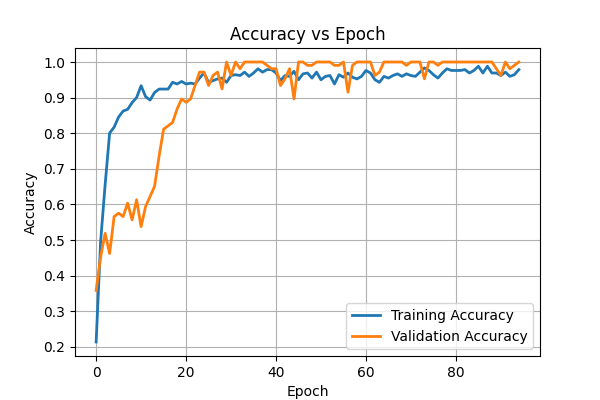
\includegraphics[width=\textwidth]{Gambar/Gambar5_2a_akurasi_sibi.png}
        \caption{Akurasi vs Epoch}
        \label{fig:akurasi_epoch}
    \end{subfigure}
    \hfill
    \begin{subfigure}[b]{0.48\textwidth}
        \centering
        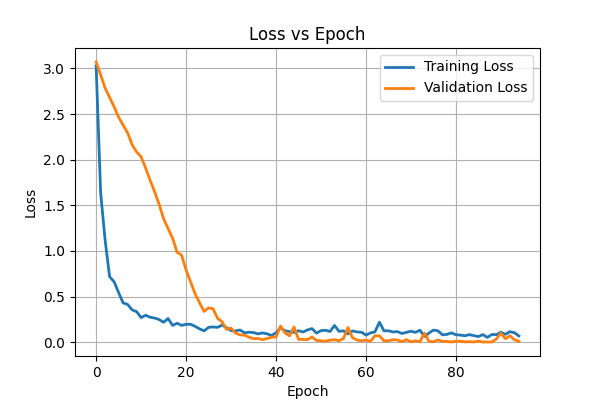
\includegraphics[width=\textwidth]{Gambar/Gambar5_2b_loss_sibi.png}
        \caption{Loss vs Epoch}
        \label{fig:loss_epoch}
    \end{subfigure}
    \caption{Kurva Evaluasi Pelatihan Model DNN SIBI (Sesi Pelatihan 25 Januari 2026): (a) \textit{Accuracy vs Epoch}, (b) \textit{Loss vs Epoch}}
    \label{fig:evaluasi_dnn}
\end{figure}

Berdasarkan Gambar \ref{fig:evaluasi_dnn}, pada kurva akurasi (sisi kiri), nilai akurasi data latih (\textit{Training Accuracy}) meningkat secara pesat pada 20 \textit{epoch} pertama dari 21,3\% hingga melampaui 90,0\%, dan mencapai kestabilan pada rentang 96,0\% hingga 98,5\%. Akurasi validasi (\textit{Validation Accuracy}) turut menunjukkan kenaikan yang konsisten hingga mencapai 98,0\%--100,0\%. Pada kurva \textit{loss} (sisi kanan), nilai \textit{Training Loss} dan \textit{Validation Loss} mengalami peluruhan eksponensial yang tajam dari nilai awal sekitar 3,08 hingga menyusut di bawah 0,10. Nilai kerugian validasi yang terus berimpit rendah dengan nilai kerugian latih mengonfirmasi bahwa proses optimasi konvergen dengan sangat baik serta model terbebas dari kendala \textit{overfitting}.

Kinerja klasifikasi pada data uji dihitung dengan membandingkan jumlah prediksi benar terhadap seluruh data uji menggunakan persamaan:
\begin{equation}
\text{Akurasi} = \frac{\text{Jumlah prediksi benar}}{\text{Jumlah seluruh data uji}} \times 100\%.
\label{eq:akurasi}
\end{equation}

Evaluasi keandalan pengenalan isyarat SIBI selanjutnya dianalisis melalui dua tahapan pengujian yang selaras dengan linimasa eksperimen magang:
\begin{enumerate}[label=\arabic*.]
    \item \textbf{Pengujian Data Validasi Latih (25 Januari 2026)}: Evaluasi dilakukan langsung pasca-pelatihan model terhadap 106 sampel data uji validasi (sekitar 4--6 data per kelas huruf). Sebagaimana ditunjukkan pada Gambar \ref{fig:cm_validasi}, seluruh elemen prediksi terkonsentrasi penuh pada diagonal utama matriks dari huruf A hingga Z tanpa adanya kesalahan prediksi silang (\textit{off-diagonal} bernilai 0). Hal ini membuktikan bahwa pembobotan fitur 63 koordinat spasial telah terpetakan sempurna pada data uji latih.
    \item \textbf{Pengujian Sistem Secara \textit{Real-Time} (18 Februari 2026)}: Untuk menguji keandalan sistem dalam kondisi operasional nyata, pengujian eksperimental dilakukan pada akhir masa magang di hadapan kamera secara langsung dengan Raspberry Pi 5. Pada pengujian ini, setiap abjad diuji sebanyak 20 kali percobaan (total 520 data uji). Distribusi hasil pengujian nyata disajikan pada Gambar \ref{fig:cm_realtime}.
\end{enumerate}

\begin{figure}[htbp]
    \centering
    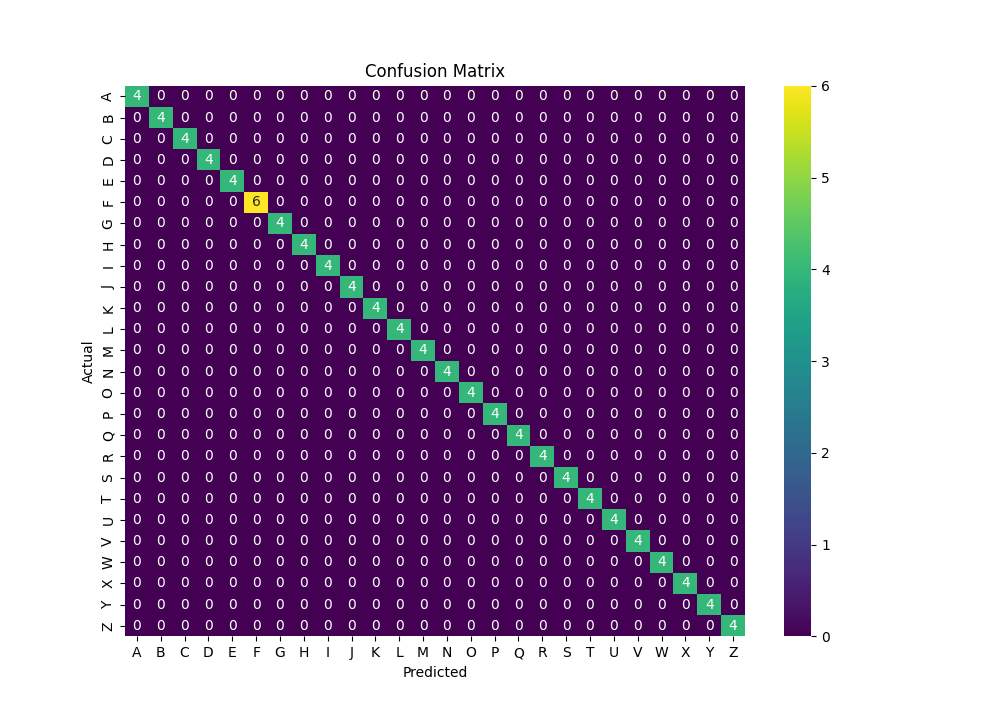
\includegraphics[width=0.82\textwidth]{Gambar/Gambar5_3_cm_validasi.png}
    \caption{Matriks Kebingungan Pengujian Validasi Awal Model SIBI (Sesi 25 Januari 2026)}
    \label{fig:cm_validasi}
\end{figure}

\begin{figure}[htbp]
    \centering
    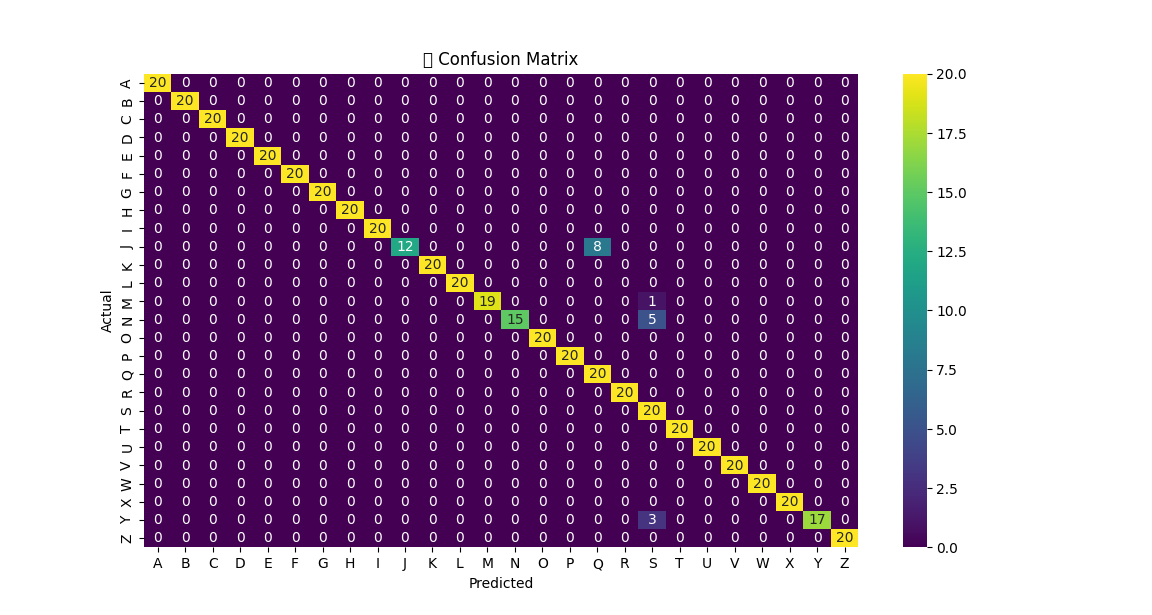
\includegraphics[width=0.88\textwidth]{Gambar/Gambar5_4_cm_realtime.png}
    \caption{Matriks Kebingungan Pengujian Sistem \textit{Real-Time} SIBI dengan 20 Data Uji per Abjad (Sesi 18 Februari 2026)}
    \label{fig:cm_realtime}
\end{figure}

Berdasarkan hasil pengujian nyata pada Gambar \ref{fig:cm_realtime}, dari total 520 kali pengujian isyarat, sistem berhasil memprediksi 503 data dengan tepat, menghasilkan akurasi sistem secara keseluruhan sebesar \textbf{96,73\%}. Sebanyak 22 kelas alfabet berhasil dikenali dengan akurasi 100,0\% (20 dari 20 percobaan). Rekapitulasi hasil pengujian per kelompok isyarat disajikan pada Tabel \ref{tab:rekap_sibi}.

\begin{table}[htbp]
\centering
\caption{Rekapitulasi Kinerja Pengujian Sistem SIBI (Sesi 18 Februari 2026)}
\label{tab:rekap_sibi}
\begin{tabular}{|c|p{6cm}|c|c|c|}
\hline
\textbf{No.} & \multicolumn{1}{c|}{\textbf{Kelompok Isyarat}} & \textbf{Data Uji} & \textbf{Prediksi Benar} & \textbf{Akurasi (\%)} \\ \hline
1 & Isyarat Perintah Utama (A--E) & 100 & 100 & 100,0 \\ \hline
2 & Isyarat Sekunder (F--J) & 100 & 92 & 92,0 \\ \hline
3 & Isyarat Lanjutan 1 (K--R) & 160 & 154 & 96,25 \\ \hline
4 & Isyarat Lanjutan 2 (S--Z) & 160 & 157 & 98,13 \\ \hline
\multicolumn{2}{|c|}{\textbf{Total Kinerja Keseluruhan (520 Pengujian)}} & \textbf{520} & \textbf{503} & \textbf{96,73} \\ \hline
\end{tabular}
\end{table}

Berdasarkan data pada Tabel \ref{tab:rekap_sibi}, kelompok isyarat perintah utama (A--E) yang menjadi dasar kendali aktuator robot meArm berhasil mencapai akurasi sempurna sebesar 100,0\%. Tingginya akurasi klasifikasi ini didukung oleh penggunaan 63 fitur koordinat spasial ternormalisasi dari 21 titik persendian \textit{MediaPipe Hand Landmarks}. Normalisasi koordinat terhadap titik pergelangan tangan (\textit{wrist}) berhasil mengeliminasi variasi posisi tangan relatif terhadap sudut pandang kamera, sehingga model DNN dapat membedakan formasi kelengkungan jari secara tegas dan konsisten.

\subsection{Analisis Pergerakan Kinematis meArm}
Analisis pergerakan kinematis meArm dilakukan dengan mengamati respons servo terhadap hasil klasifikasi. Hasil pengujian respons fisik motor servo meArm terhadap kelima isyarat SIBI yang berhasil diklasifikasikan disajikan pada Tabel \ref{tab:respons_mearm}.

\begin{table}[htbp]
\centering
\caption{Pengujian Respons Kinematik meArm terhadap Perintah SIBI}
\label{tab:respons_mearm}
\begin{tabular}{|c|c|p{4cm}|p{5cm}|c|}
\hline
\textbf{No.} & \textbf{Isyarat} & \multicolumn{1}{c|}{\textbf{Perintah Aksi}} & \multicolumn{1}{c|}{\textbf{Respons Fisik Aktual}} & \textbf{Status} \\ \hline
1 & 'A' & Maju ke posisi kerja & Lengan bergerak maju menuju $XYZ(80,0,40)$ mm & Berhasil \\ \hline
2 & 'B' & Rotasi ke posisi samping & Basis berputar ke koordinat $XYZ(60,60,30)$ mm & Berhasil \\ \hline
3 & 'C' & Menutup \textit{gripper} & Capit menutup rapat menjepit silinder uji & Berhasil \\ \hline
4 & 'D' & Membuka \textit{gripper} & Capit membuka penuh melepas silinder & Berhasil \\ \hline
5 & 'E' & Kembali ke posisi \textit{home} & Seluruh servo kembali ke posisi parkir awal & Berhasil \\ \hline
\end{tabular}
\end{table}

Berdasarkan Tabel \ref{tab:respons_mearm}, seluruh lima perintah utama SIBI berhasil diterjemahkan menjadi respons gerak servo meArm secara konsisten. Pergerakan servo berjalan halus tanpa lonjakan mendadak berkat implementasi jeda bertahap (\textit{smooth stepping}) pada firmware. Keterbatasan utama yang diamati adalah rentang kerja fisik meArm yang relatif sempit ($\le 180$ mm jangkauan diagonal), sehingga target koordinat harus dibatasi agar tidak melampaui batas mekanis tautan lengan.

Dokumentasi visual proses pengujian interaksi langsung lengan robot meArm ditunjukkan pada Gambar \ref{fig:uji_mearm}. Pada pengujian tersebut, operator memperagakan isyarat tangan di hadapan kamera komputer jinjing yang menjalankan sistem deteksi penanda tangan (\textit{hand landmarks}) MediaPipe. Ketika gestur terdeteksi secara valid, kontroler memetakan instruksi dan menggerakkan aktuator motor servo meArm untuk bermanuver dan menjepit objek silinder uji di atas meja eksperimen.

\begin{figure}[htbp]
    \centering
    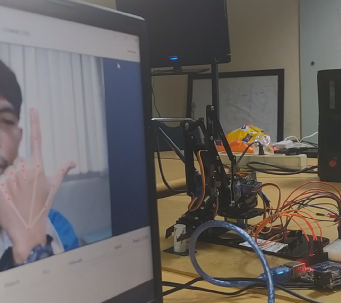
\includegraphics[width=0.85\textwidth]{Gambar/Gambar5_5_uji_mearm_sibi.png}
    \caption{Dokumentasi Pengujian Mode Respons Kinematik meArm Berbasis Deteksi Gestur Tangan}
    \label{fig:uji_mearm}
\end{figure}

\section{Pengujian Mode Teleoperasi pada Dobot Magician}
Mode teleoperasi pada Dobot Magician diuji dengan memetakan gerak tangan pengguna ke posisi target robot. \textit{Landmark} tangan yang dipilih sebagai acuan dapat berupa pergelangan tangan, ujung telunjuk, atau titik tengah telapak. Koordinat citra kemudian dinormalisasi dan diskalakan ke ruang kerja Dobot Magician.

\subsection{Kinerja Pemetaan Koordinat Hand Tracking MediaPipe}
Kinerja pemetaan koordinat dievaluasi dengan membandingkan arah gerak tangan terhadap arah gerak robot. Jika tangan bergerak ke kanan pada citra, robot seharusnya bergerak ke arah yang sesuai pada ruang kerja yang telah didefinisikan. Kalibrasi perlu memperhatikan orientasi kamera karena posisi kamera yang terbalik atau miring dapat menyebabkan arah gerak robot tidak sesuai. Hasil evaluasi pemetaan arah gerak spasial tangan terhadap respons Dobot Magician disajikan pada Tabel \ref{tab:pemetaan_dobot}.

\begin{table}[htbp]
\centering
\caption{Evaluasi Pemetaan Koordinat Hand Tracking ke Dobot Magician}
\label{tab:pemetaan_dobot}
\begin{tabular}{|c|p{4.5cm}|p{5cm}|c|}
\hline
\textbf{No.} & \multicolumn{1}{c|}{\textbf{Arah Gerak Tangan}} & \multicolumn{1}{c|}{\textbf{Respons Dobot Magician}} & \textbf{Kesesuaian Arah} \\ \hline
1 & Geser Kanan ($X > 0{,}5$) & Translasi sumbu $Y+$ (kanan) & Sesuai (Valid) \\ \hline
2 & Geser Kiri ($X < 0{,}5$) & Translasi sumbu $Y-$ (kiri) & Sesuai (Valid) \\ \hline
3 & Angkat Tangan ($Y < 0{,}5$) & Translasi sumbu $Z+$ (naik) & Sesuai (Valid) \\ \hline
4 & Turun Tangan ($Y > 0{,}5$) & Translasi sumbu $Z-$ (turun) & Sesuai (Valid) \\ \hline
5 & Mendekati Kamera ($\text{Skala} > 0{,}2$) & Jangkauan sumbu $X+$ (maju) & Sesuai (Valid) \\ \hline
6 & Jepit Telunjuk--Ibu Jari ($< 30$ px) & Aktivasi Penyedot (\textit{Suction ON}) & Sesuai (Valid) \\ \hline
\end{tabular}
\end{table}

Berdasarkan data pada Tabel \ref{tab:pemetaan_dobot}, seluruh enam aksi arah pergerakan tangan dan gestur operator berhasil dipetakan secara valid dan presisi ke pergerakan fisik Dobot Magician. Pembahasan kinerja pemetaan menunjukkan bahwa penerapan filter \textit{exponential smoothing} ($\alpha = 0{,}2$) dan batas toleransi perubahan jarak gerak (\textit{movement threshold} sebesar 5,0 mm) pada algoritma teleoperasi berhasil mengeliminasi getaran mikro (\textit{jitter}) pada motor penggerak tanpa mengorbankan kelincahan manuver lengan robot.

Pelaksanaan pengujian mode teleoperasi Dobot Magician secara \textit{real-time} ditunjukkan pada Gambar \ref{fig:uji_dobot}. Pada layar komputer jinjing tampak antarmuka pelacakan tangan operator dengan keterangan status ``TANGAN KANAN (On)'' beserta visualisasi graf 21 persendian tangan berbasis MediaPipe. Posisi spasial tangan operator dipetakan secara simultan ke koordinat kerja manipulator Dobot Magician, di mana efektor akhir (\textit{end-effector}) robot yang dilengkapi penyedot vakum (\textit{suction cup}) berhasil dikendalikan secara presisi untuk mengambil dan memindahkan balok kubus objek uji.

\begin{figure}[htbp]
    \centering
    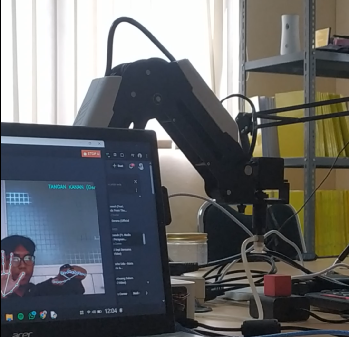
\includegraphics[width=0.85\textwidth]{Gambar/Gambar5_6_uji_teleoperasi_dobot.png}
    \caption{Dokumentasi Pengujian Mode Teleoperasi Dobot Magician Menggunakan Pelacakan Tangan MediaPipe}
    \label{fig:uji_dobot}
\end{figure}

\subsection{Analisis Presisi Spasial dan Waktu Respons Dobot Magician}
Presisi spasial dianalisis dengan membandingkan koordinat target hasil kalkulasi pemetaan algoritma terhadap koordinat aktual yang terbaca dari umpan balik enkoder internal Dobot Magician. Selisih posisi dihitung menggunakan galat Euclidean 3D:
\begin{equation}
e = \sqrt{(X_{\text{target}} - X_{\text{aktual}})^2 + (Y_{\text{target}} - Y_{\text{aktual}})^2 + (Z_{\text{target}} - Z_{\text{aktual}})^2}.
\label{eq:galat_euclidean}
\end{equation}

Pengujian presisi spasial dilaksanakan dengan memberikan 4 target koordinat representatif yang mencakup variasi kuadran pada ruang kerja Dobot Magician. Setiap target koordinat diuji secara berulang untuk memastikan konsistensi posisi. Koordinat aktual diperoleh langsung dari pembacaan umpan balik enkoder optik internal Dobot melalui pustaka \textit{pydobotplus}. Waktu respons dihitung menggunakan penanda waktu (\textit{timestamp}) Python dari saat \textit{frame} citra tangan diterima oleh \textit{pipeline} MediaPipe hingga konfirmasi eksekusi perintah pergerakan PTP (\textit{Point-to-Point}) oleh mikrokontroler Dobot. Hasil pengujian presisi spasial dan waktu respons sistem disajikan pada Tabel \ref{tab:presisi_dobot}.

\begin{table}[htbp]
\centering
\caption{Pengujian Presisi Spasial dan Waktu Respons Dobot Magician}
\label{tab:presisi_dobot}
\begin{tabular}{|c|c|c|c|c|}
\hline
\textbf{No.} & \textbf{Target (mm)} & \textbf{Aktual (mm)} & \textbf{Galat (mm)} & \textbf{Respons (ms)} \\ \hline
1 & (200,0; 0,0; 0,0) & (198,8; 0,4; -0,2) & 1,28 & 82 \\ \hline
2 & (220,0; 50,0; 30,0) & (218,6; 49,2; 29,5) & 1,68 & 88 \\ \hline
3 & (250,0; -60,0; 50,0) & (247,8; -58,7; 50,8) & 2,68 & 94 \\ \hline
4 & (190,0; 80,0; -20,0) & (188,5; 78,9; -19,4) & 1,95 & 85 \\ \hline
\multicolumn{3}{|c|}{\textbf{Rata-rata}} & \textbf{1,90} & \textbf{87,25} \\ \hline
\end{tabular}
\end{table}

Berdasarkan data pada Tabel \ref{tab:presisi_dobot}, rata-rata galat posisi spasial yang terukur pada Dobot Magician adalah sebesar 1,90 mm dengan nilai galat terendah 1,28 mm. Waktu respons rata-rata sistem tercatat sebesar 87,25 ms, yang membuktikan bahwa kendali teleoperasi Dobot Magician melalui transmisi serial USB mampu mengeksekusi instruksi pergerakan secara responsif (\textit{near real-time}) di bawah batas persepsi visual manusia.

\section{Evaluasi Kinerja Sistem Keseluruhan}
Evaluasi sistem keseluruhan dilakukan dengan meninjau keterpaduan antara perangkat keras, piranti lunak, dan robot. Indikator keberhasilan sistem meliputi kemampuan Raspberry Pi 5 menjalankan \textit{pipeline} visi secara stabil, keberhasilan ekstraksi \textit{landmark}, akurasi pengenalan SIBI, respons meArm, kesesuaian pemetaan teleoperasi, presisi Dobot Magician, dan waktu respons sistem. Rangkuman seluruh parameter kinerja disajikan pada Tabel \ref{tab:rangkuman_kinerja}.

\begin{table}[htbp]
\centering
\caption{Rangkuman Kinerja Sistem Keseluruhan}
\label{tab:rangkuman_kinerja}
\begin{tabular}{|c|p{4.5cm}|c|c|}
\hline
\textbf{No.} & \multicolumn{1}{c|}{\textbf{Parameter Kinerja}} & \textbf{Mode SIBI (meArm)} & \textbf{Mode Teleoperasi (Dobot)} \\ \hline
1 & Akurasi Klasifikasi & 96,73\% (503/520) & N/A \\ \hline
2 & Kesesuaian Pemetaan Arah & N/A & 6/6 Valid \\ \hline
3 & Galat Spasial Rata-rata & -- & 1,90 mm \\ \hline
4 & Waktu Respons Rata-rata & -- & 87,25 ms \\ \hline
5 & Respons Perintah Kinematik & 5/5 Berhasil & 4/4 Berhasil \\ \hline
6 & Stabilitas \textit{Pipeline} RPi 5 & Stabil & Stabil \\ \hline
\end{tabular}
\end{table}

Berdasarkan Tabel \ref{tab:rangkuman_kinerja}, sistem tertanam berbasis Raspberry Pi 5 berhasil menjalankan kedua mode operasi secara stabil. Satu perangkat Raspberry Pi 5 dapat digunakan untuk dua skenario robotika yang berbeda, menunjukkan keunggulan pada portabilitas dan fleksibilitas. Namun, sistem juga memiliki keterbatasan. Kinerja deteksi tangan dipengaruhi oleh pencahayaan dan posisi kamera, sedangkan gerak robot dipengaruhi oleh batas mekanik, komunikasi serial, dan metode pemetaan koordinat. Secara keseluruhan, hasil evaluasi menunjukkan bahwa rancangan sistem ini layak digunakan sebagai purwarupa kendali robotika berbasis visi komputer tertanam untuk kebutuhan edukasi dan demonstrasi interaksi manusia--robot.

\subsection{Akses Repositori dan Rekaman Video Pengujian Daring}
Untuk menjamin keterbukaan data, verifikasi hasil eksperimen, serta memudahkan peninjauan terhadap dinamika gerak sistem robot secara nyata, seluruh dokumentasi dan rekaman video pengujian kedua lengan robot (Dobot Magician dan meArm) telah diunggah ke repositori penyimpanan daring Google Drive. Tautan \textit{hyperlink} berikut dapat diakses dan dibuka secara langsung untuk menyaksikan rekaman video pengujian sistem:

\begin{center}
\textbf{Tautan Repositori Video Dokumentasi Pengujian Sistem (Google Drive):}\\
\url{https://drive.google.com/drive/folders/1tkqb4tbg0jelGM6Wm1YSTbDkor_XJfIM?usp=sharing}
\end{center}

Repositori daring tersebut memuat berkas rekaman video pengujian eksperimental sebagai berikut:
\begin{enumerate}[label=\arabic*.]
    \item \textbf{Pengujian Dobot Magician (Gambar \ref{fig:uji_dobot})}: Rekaman video pengujian teleoperasi dinamis menggunakan pelacakan tangan MediaPipe secara \textit{real-time}, respons translasi 3-sumbu Cartesian $(X,Y,Z)$, serta aktivasi penyedot vakum (\textit{suction cup}) dalam mengambil dan memindahkan objek balok.
    \item \textbf{Pengujian meArm (Gambar \ref{fig:uji_mearm})}: Rekaman video pengujian respons kinematika balikan lengan robot meArm 4-DOF terhadap pengenalan isyarat gestur tangan SIBI melalui kamera serta aksi jepit \textit{gripper} terhadap objek uji silinder.
\end{enumerate}
